\documentclass[twoside]{book}

% Packages required by doxygen
\usepackage{calc}
\usepackage{doxygen}
\usepackage{graphicx}
\usepackage[utf8]{inputenc}
\usepackage{makeidx}
\usepackage{multicol}
\usepackage{multirow}
\usepackage{textcomp}
\usepackage[table]{xcolor}

% Font selection
\usepackage[T1]{fontenc}
\usepackage{mathptmx}
\usepackage[scaled=.90]{helvet}
\usepackage{courier}
\usepackage{amssymb}
\usepackage{sectsty}
\renewcommand{\familydefault}{\sfdefault}
\allsectionsfont{%
  \fontseries{bc}\selectfont%
  \color{darkgray}%
}
\renewcommand{\DoxyLabelFont}{%
  \fontseries{bc}\selectfont%
  \color{darkgray}%
}

% Page & text layout
\usepackage{geometry}
\geometry{%
  a4paper,%
  top=2.5cm,%
  bottom=2.5cm,%
  left=2.5cm,%
  right=2.5cm%
}
\tolerance=750
\hfuzz=15pt
\hbadness=750
\setlength{\emergencystretch}{15pt}
\setlength{\parindent}{0cm}
\setlength{\parskip}{0.2cm}
\makeatletter
\renewcommand{\paragraph}{%
  \@startsection{paragraph}{4}{0ex}{-1.0ex}{1.0ex}{%
    \normalfont\normalsize\bfseries\SS@parafont%
  }%
}
\renewcommand{\subparagraph}{%
  \@startsection{subparagraph}{5}{0ex}{-1.0ex}{1.0ex}{%
    \normalfont\normalsize\bfseries\SS@subparafont%
  }%
}
\makeatother

% Headers & footers
\usepackage{fancyhdr}
\pagestyle{fancyplain}
\fancyhead[LE]{\fancyplain{}{\bfseries\thepage}}
\fancyhead[CE]{\fancyplain{}{}}
\fancyhead[RE]{\fancyplain{}{\bfseries\leftmark}}
\fancyhead[LO]{\fancyplain{}{\bfseries\rightmark}}
\fancyhead[CO]{\fancyplain{}{}}
\fancyhead[RO]{\fancyplain{}{\bfseries\thepage}}
\fancyfoot[LE]{\fancyplain{}{}}
\fancyfoot[CE]{\fancyplain{}{}}
\fancyfoot[RE]{\fancyplain{}{\bfseries\scriptsize Generated on Tue Nov 26 2013 11:21:15 for Example JS Project by Doxygen }}
\fancyfoot[LO]{\fancyplain{}{\bfseries\scriptsize Generated on Tue Nov 26 2013 11:21:15 for Example JS Project by Doxygen }}
\fancyfoot[CO]{\fancyplain{}{}}
\fancyfoot[RO]{\fancyplain{}{}}
\renewcommand{\footrulewidth}{0.4pt}
\renewcommand{\chaptermark}[1]{%
  \markboth{#1}{}%
}
\renewcommand{\sectionmark}[1]{%
  \markright{\thesection\ #1}%
}

% Indices & bibliography
\usepackage{natbib}
\usepackage[titles]{tocloft}
\setcounter{tocdepth}{3}
\setcounter{secnumdepth}{5}
\makeindex

% Hyperlinks (required, but should be loaded last)
\usepackage{ifpdf}
\ifpdf
  \usepackage[pdftex,pagebackref=true]{hyperref}
\else
  \usepackage[ps2pdf,pagebackref=true]{hyperref}
\fi
\hypersetup{%
  colorlinks=true,%
  linkcolor=blue,%
  citecolor=blue,%
  unicode%
}

% Custom commands
\newcommand{\clearemptydoublepage}{%
  \newpage{\pagestyle{empty}\cleardoublepage}%
}


%===== C O N T E N T S =====

\begin{document}

% Titlepage & ToC
\hypersetup{pageanchor=false}
\pagenumbering{roman}
\begin{titlepage}
\vspace*{7cm}
\begin{center}%
{\Large Example J\-S Project }\\
\vspace*{1cm}
{\large Generated by Doxygen 1.8.4}\\
\vspace*{0.5cm}
{\small Tue Nov 26 2013 11:21:15}\\
\end{center}
\end{titlepage}
\clearemptydoublepage
\tableofcontents
\clearemptydoublepage
\pagenumbering{arabic}
\hypersetup{pageanchor=true}

%--- Begin generated contents ---
\chapter{Hierarchical Index}
\section{Class Hierarchy}
This inheritance list is sorted roughly, but not completely, alphabetically\-:\begin{DoxyCompactList}
\item Animation\begin{DoxyCompactList}
\item \contentsline{section}{about\-\_\-us\-\_\-module\-:\-:read\-More\-\_\-hide}{\pageref{classabout__us__module_1_1readMore__hide}}{}
\item \contentsline{section}{about\-\_\-us\-\_\-module\-:\-:read\-More\-\_\-show}{\pageref{classabout__us__module_1_1readMore__show}}{}
\item \contentsline{section}{about\-\_\-us\-\_\-module\-:\-:team\-Bio\-\_\-hide}{\pageref{classabout__us__module_1_1teamBio__hide}}{}
\item \contentsline{section}{about\-\_\-us\-\_\-module\-:\-:team\-Bio\-\_\-show}{\pageref{classabout__us__module_1_1teamBio__show}}{}
\item \contentsline{section}{example\-\_\-module\-:\-:team\-Bio\-\_\-hide}{\pageref{classexample__module_1_1teamBio__hide}}{}
\end{DoxyCompactList}
\item Controller\begin{DoxyCompactList}
\item \contentsline{section}{about\-\_\-us\-\_\-module\-:\-:img\-Gallery\-Controller}{\pageref{classabout__us__module_1_1imgGalleryController}}{}
\item \contentsline{section}{about\-\_\-us\-\_\-module\-:\-:more\-Info\-Controller}{\pageref{classabout__us__module_1_1moreInfoController}}{}
\item \contentsline{section}{about\-\_\-us\-\_\-module\-:\-:sidebar\-Controller}{\pageref{classabout__us__module_1_1sidebarController}}{}
\item \contentsline{section}{about\-\_\-us\-\_\-module\-:\-:team\-Bio\-Controller}{\pageref{classabout__us__module_1_1teamBioController}}{}
\end{DoxyCompactList}
\item Directive\begin{DoxyCompactList}
\item \contentsline{section}{about\-\_\-us\-\_\-module\-:\-:sticky\-Nav}{\pageref{classabout__us__module_1_1stickyNav}}{}
\end{DoxyCompactList}
\item Factory\begin{DoxyCompactList}
\item \contentsline{section}{about\-\_\-us\-\_\-module\-:\-:team\-Member\-Factory}{\pageref{classabout__us__module_1_1teamMemberFactory}}{}
\end{DoxyCompactList}
\item promise\begin{DoxyCompactList}
\item \contentsline{section}{about\-\_\-us\-\_\-module\-:\-:team\-Member\-Factory}{\pageref{classabout__us__module_1_1teamMemberFactory}}{}
\end{DoxyCompactList}
\end{DoxyCompactList}

\chapter{Class Index}
\section{Class List}
Here are the classes, structs, unions and interfaces with brief descriptions\-:\begin{DoxyCompactList}
\item\contentsline{section}{\hyperlink{classabout__us__module_1_1imgGalleryController}{about\-\_\-us\-\_\-module\-::img\-Gallery\-Controller} }{\pageref{classabout__us__module_1_1imgGalleryController}}{}
\item\contentsline{section}{\hyperlink{classabout__us__module_1_1moreInfoController}{about\-\_\-us\-\_\-module\-::more\-Info\-Controller} }{\pageref{classabout__us__module_1_1moreInfoController}}{}
\item\contentsline{section}{\hyperlink{classabout__us__module_1_1readMore__hide}{about\-\_\-us\-\_\-module\-::read\-More\-\_\-hide} }{\pageref{classabout__us__module_1_1readMore__hide}}{}
\item\contentsline{section}{\hyperlink{classabout__us__module_1_1readMore__show}{about\-\_\-us\-\_\-module\-::read\-More\-\_\-show} }{\pageref{classabout__us__module_1_1readMore__show}}{}
\item\contentsline{section}{\hyperlink{classabout__us__module_1_1sidebarController}{about\-\_\-us\-\_\-module\-::sidebar\-Controller} }{\pageref{classabout__us__module_1_1sidebarController}}{}
\item\contentsline{section}{\hyperlink{classabout__us__module_1_1stickyNav}{about\-\_\-us\-\_\-module\-::sticky\-Nav} }{\pageref{classabout__us__module_1_1stickyNav}}{}
\item\contentsline{section}{\hyperlink{classabout__us__module_1_1teamBio__hide}{about\-\_\-us\-\_\-module\-::team\-Bio\-\_\-hide} }{\pageref{classabout__us__module_1_1teamBio__hide}}{}
\item\contentsline{section}{\hyperlink{classabout__us__module_1_1teamBio__show}{about\-\_\-us\-\_\-module\-::team\-Bio\-\_\-show} }{\pageref{classabout__us__module_1_1teamBio__show}}{}
\item\contentsline{section}{\hyperlink{classabout__us__module_1_1teamBioController}{about\-\_\-us\-\_\-module\-::team\-Bio\-Controller} }{\pageref{classabout__us__module_1_1teamBioController}}{}
\item\contentsline{section}{\hyperlink{classexample__module_1_1teamBioController}{example\-\_\-module\-::team\-Bio\-Controller} }{\pageref{classexample__module_1_1teamBioController}}{}
\item\contentsline{section}{\hyperlink{classabout__us__module_1_1teamMemberFactory}{about\-\_\-us\-\_\-module\-::team\-Member\-Factory} }{\pageref{classabout__us__module_1_1teamMemberFactory}}{}
\end{DoxyCompactList}

\chapter{Class Documentation}
\hypertarget{classabout__us__module_1_1imgGalleryController}{\section{about\-\_\-us\-\_\-module\-:\-:img\-Gallery\-Controller Class Reference}
\label{classabout__us__module_1_1imgGalleryController}\index{about\-\_\-us\-\_\-module\-::img\-Gallery\-Controller@{about\-\_\-us\-\_\-module\-::img\-Gallery\-Controller}}
}
Inheritance diagram for about\-\_\-us\-\_\-module\-:\-:img\-Gallery\-Controller\-:\begin{figure}[H]
\begin{center}
\leavevmode
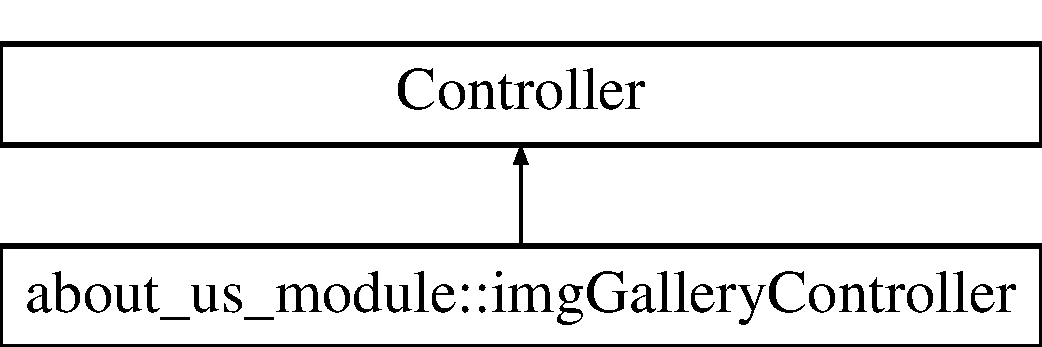
\includegraphics[height=2.000000cm]{classabout__us__module_1_1imgGalleryController}
\end{center}
\end{figure}
\subsection*{Public Member Functions}
\begin{DoxyCompactItemize}
\item 
\hypertarget{classabout__us__module_1_1imgGalleryController_a76177ef60341ea216545e3a0cbb01f18}{{\bfseries go\-To} (index)}\label{classabout__us__module_1_1imgGalleryController_a76177ef60341ea216545e3a0cbb01f18}

\item 
\hypertarget{classabout__us__module_1_1imgGalleryController_a057f6cc2df7e2e59c0dbe09dbf272ba7}{{\bfseries click\-Thumb} (index)}\label{classabout__us__module_1_1imgGalleryController_a057f6cc2df7e2e59c0dbe09dbf272ba7}

\item 
\hypertarget{classabout__us__module_1_1imgGalleryController_acdedbf295d011139daf7a9fd6aa7b590}{{\bfseries next} ()}\label{classabout__us__module_1_1imgGalleryController_acdedbf295d011139daf7a9fd6aa7b590}

\item 
\hypertarget{classabout__us__module_1_1imgGalleryController_aea88dd40e7708df4c3d85a5508f6b5bb}{{\bfseries prev} ()}\label{classabout__us__module_1_1imgGalleryController_aea88dd40e7708df4c3d85a5508f6b5bb}

\end{DoxyCompactItemize}
\subsection*{Public Attributes}
\begin{DoxyCompactItemize}
\item 
\hypertarget{classabout__us__module_1_1imgGalleryController_a5a314bbda4c1a9a9cd407c776e5db554}{{\bfseries img\-Gallery\-Text}}\label{classabout__us__module_1_1imgGalleryController_a5a314bbda4c1a9a9cd407c776e5db554}

\item 
\hypertarget{classabout__us__module_1_1imgGalleryController_a73dfed5ee9c4af1ba32f07678841ad5d}{{\bfseries active}}\label{classabout__us__module_1_1imgGalleryController_a73dfed5ee9c4af1ba32f07678841ad5d}

\item 
\hypertarget{classabout__us__module_1_1imgGalleryController_adcee86e51598901ab32eea0c5352902b}{{\bfseries active\-Index}}\label{classabout__us__module_1_1imgGalleryController_adcee86e51598901ab32eea0c5352902b}

\item 
\hypertarget{classabout__us__module_1_1imgGalleryController_ac643f17760b71339b67e480f9acdd314}{{\bfseries youtube}}\label{classabout__us__module_1_1imgGalleryController_ac643f17760b71339b67e480f9acdd314}

\end{DoxyCompactItemize}


The documentation for this class was generated from the following file\-:\begin{DoxyCompactItemize}
\item 
about-\/us.\-js\end{DoxyCompactItemize}

\hypertarget{classabout__us__module_1_1moreInfoController}{\section{about\-\_\-us\-\_\-module\-:\-:more\-Info\-Controller Class Reference}
\label{classabout__us__module_1_1moreInfoController}\index{about\-\_\-us\-\_\-module\-::more\-Info\-Controller@{about\-\_\-us\-\_\-module\-::more\-Info\-Controller}}
}
Inheritance diagram for about\-\_\-us\-\_\-module\-:\-:more\-Info\-Controller\-:\begin{figure}[H]
\begin{center}
\leavevmode
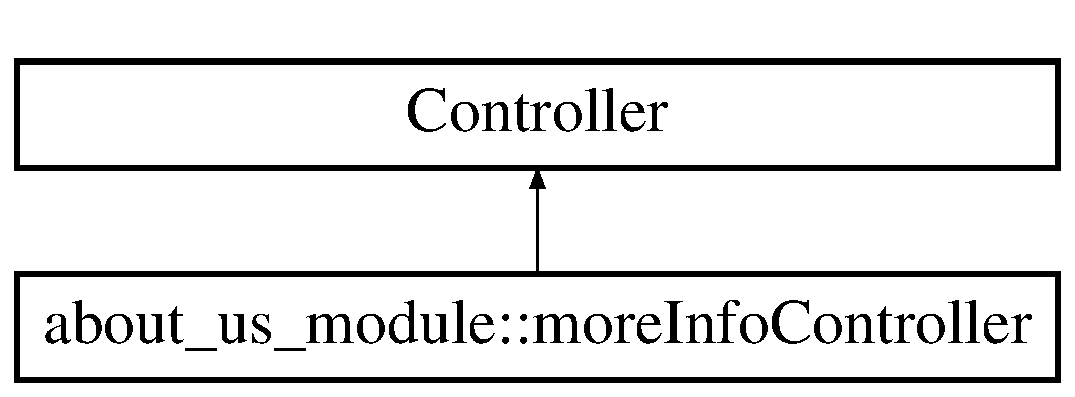
\includegraphics[height=2.000000cm]{classabout__us__module_1_1moreInfoController}
\end{center}
\end{figure}
\subsection*{Public Member Functions}
\begin{DoxyCompactItemize}
\item 
\hypertarget{classabout__us__module_1_1moreInfoController_a316ace3a6be8c89e097d7459224f213d}{{\bfseries toggle\-Box} ()}\label{classabout__us__module_1_1moreInfoController_a316ace3a6be8c89e097d7459224f213d}

\end{DoxyCompactItemize}
\subsection*{Public Attributes}
\begin{DoxyCompactItemize}
\item 
\hypertarget{classabout__us__module_1_1moreInfoController_affa9bd2cbbc263c93ee00ec40e1051c9}{{\bfseries is\-Box\-Open}}\label{classabout__us__module_1_1moreInfoController_affa9bd2cbbc263c93ee00ec40e1051c9}

\item 
\hypertarget{classabout__us__module_1_1moreInfoController_a27d5952fdc112f5fbab63c461955e755}{{\bfseries btn\-Label}}\label{classabout__us__module_1_1moreInfoController_a27d5952fdc112f5fbab63c461955e755}

\item 
\hypertarget{classabout__us__module_1_1moreInfoController_acfa0d4f04df2f8c6006108c6a1e7d631}{{\bfseries btn\-Arrow}}\label{classabout__us__module_1_1moreInfoController_acfa0d4f04df2f8c6006108c6a1e7d631}

\end{DoxyCompactItemize}


The documentation for this class was generated from the following file\-:\begin{DoxyCompactItemize}
\item 
about-\/us.\-js\end{DoxyCompactItemize}

\hypertarget{classabout__us__module_1_1readMore__hide}{\section{about\-\_\-us\-\_\-module\-:\-:read\-More\-\_\-hide Class Reference}
\label{classabout__us__module_1_1readMore__hide}\index{about\-\_\-us\-\_\-module\-::read\-More\-\_\-hide@{about\-\_\-us\-\_\-module\-::read\-More\-\_\-hide}}
}
Inheritance diagram for about\-\_\-us\-\_\-module\-:\-:read\-More\-\_\-hide\-:\begin{figure}[H]
\begin{center}
\leavevmode
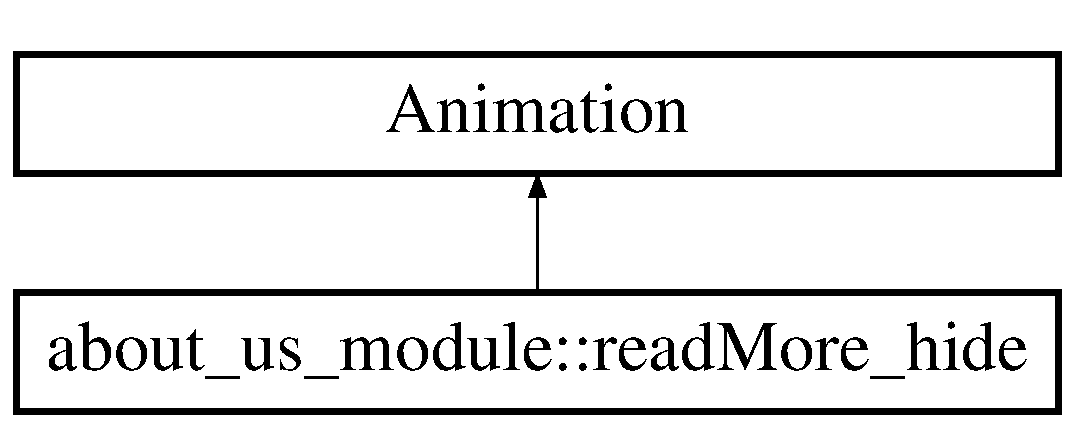
\includegraphics[height=2.000000cm]{classabout__us__module_1_1readMore__hide}
\end{center}
\end{figure}


The documentation for this class was generated from the following file\-:\begin{DoxyCompactItemize}
\item 
about-\/us.\-js\end{DoxyCompactItemize}

\hypertarget{classabout__us__module_1_1readMore__show}{\section{about\-\_\-us\-\_\-module\-:\-:read\-More\-\_\-show Class Reference}
\label{classabout__us__module_1_1readMore__show}\index{about\-\_\-us\-\_\-module\-::read\-More\-\_\-show@{about\-\_\-us\-\_\-module\-::read\-More\-\_\-show}}
}
Inheritance diagram for about\-\_\-us\-\_\-module\-:\-:read\-More\-\_\-show\-:\begin{figure}[H]
\begin{center}
\leavevmode
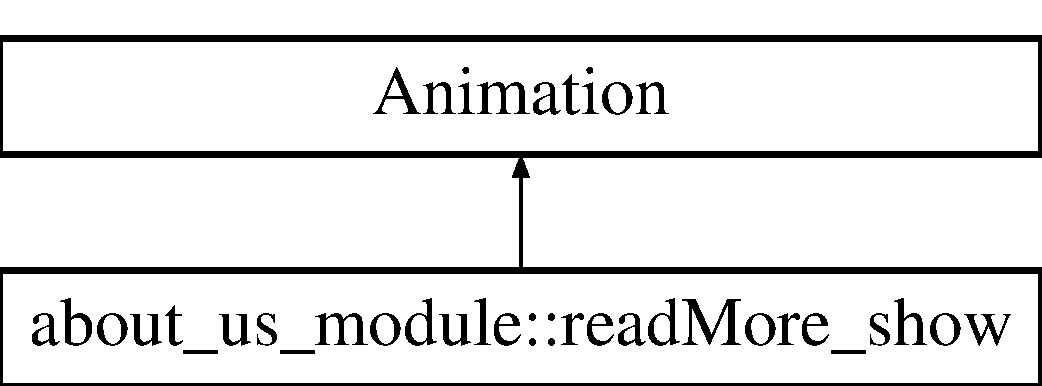
\includegraphics[height=2.000000cm]{classabout__us__module_1_1readMore__show}
\end{center}
\end{figure}


The documentation for this class was generated from the following file\-:\begin{DoxyCompactItemize}
\item 
about-\/us.\-js\end{DoxyCompactItemize}

\hypertarget{classabout__us__module_1_1sidebarController}{\section{about\-\_\-us\-\_\-module\-:\-:sidebar\-Controller Class Reference}
\label{classabout__us__module_1_1sidebarController}\index{about\-\_\-us\-\_\-module\-::sidebar\-Controller@{about\-\_\-us\-\_\-module\-::sidebar\-Controller}}
}
Inheritance diagram for about\-\_\-us\-\_\-module\-:\-:sidebar\-Controller\-:\begin{figure}[H]
\begin{center}
\leavevmode
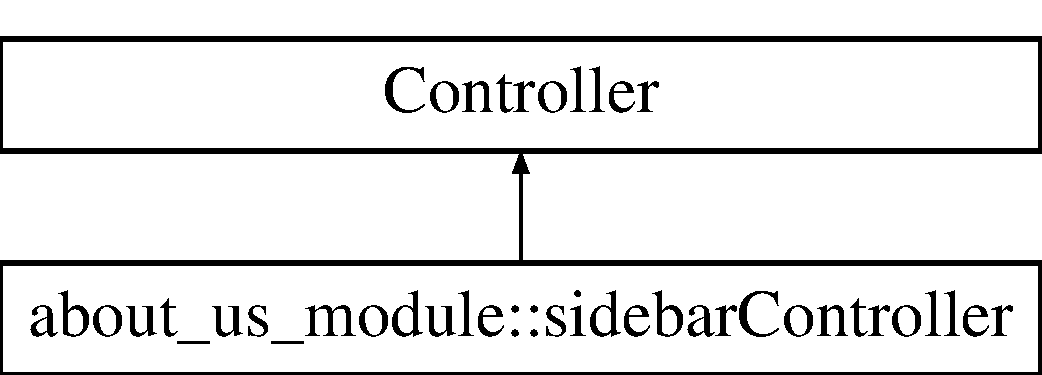
\includegraphics[height=2.000000cm]{classabout__us__module_1_1sidebarController}
\end{center}
\end{figure}
\subsection*{Public Member Functions}
\begin{DoxyCompactItemize}
\item 
\hypertarget{classabout__us__module_1_1sidebarController_a81e1f60ac857f46e7ef2503a31f60b91}{{\bfseries scroll\-To} (id)}\label{classabout__us__module_1_1sidebarController_a81e1f60ac857f46e7ef2503a31f60b91}

\end{DoxyCompactItemize}
\subsection*{Public Attributes}
\begin{DoxyCompactItemize}
\item 
\hypertarget{classabout__us__module_1_1sidebarController_a8672dd6cb1de416c842be0db0ce8397f}{{\bfseries is\-Active}}\label{classabout__us__module_1_1sidebarController_a8672dd6cb1de416c842be0db0ce8397f}

\end{DoxyCompactItemize}


The documentation for this class was generated from the following file\-:\begin{DoxyCompactItemize}
\item 
about-\/us.\-js\end{DoxyCompactItemize}

\hypertarget{classabout__us__module_1_1stickyNav}{\section{about\-\_\-us\-\_\-module\-:\-:sticky\-Nav Class Reference}
\label{classabout__us__module_1_1stickyNav}\index{about\-\_\-us\-\_\-module\-::sticky\-Nav@{about\-\_\-us\-\_\-module\-::sticky\-Nav}}
}
Inheritance diagram for about\-\_\-us\-\_\-module\-:\-:sticky\-Nav\-:\begin{figure}[H]
\begin{center}
\leavevmode
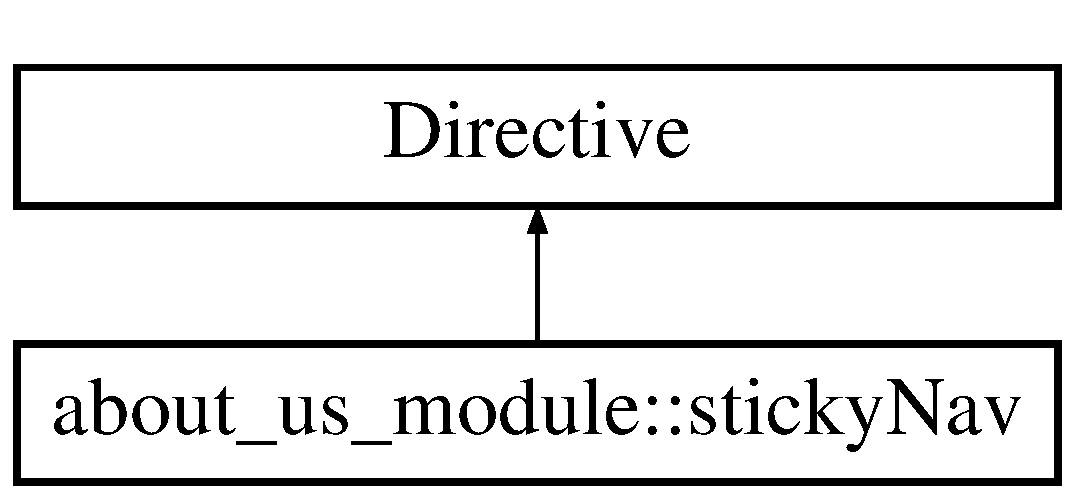
\includegraphics[height=2.000000cm]{classabout__us__module_1_1stickyNav}
\end{center}
\end{figure}
\subsection*{Public Member Functions}
\begin{DoxyCompactItemize}
\item 
\hypertarget{classabout__us__module_1_1stickyNav_a5c68df5aee987ceed270554d8d62a370}{{\bfseries sticky\-Nav} (sticky\-Start, sticky\-End)}\label{classabout__us__module_1_1stickyNav_a5c68df5aee987ceed270554d8d62a370}

\end{DoxyCompactItemize}


The documentation for this class was generated from the following file\-:\begin{DoxyCompactItemize}
\item 
about-\/us.\-js\end{DoxyCompactItemize}

\hypertarget{classabout__us__module_1_1teamBio__hide}{\section{about\-\_\-us\-\_\-module\-:\-:team\-Bio\-\_\-hide Class Reference}
\label{classabout__us__module_1_1teamBio__hide}\index{about\-\_\-us\-\_\-module\-::team\-Bio\-\_\-hide@{about\-\_\-us\-\_\-module\-::team\-Bio\-\_\-hide}}
}
Inheritance diagram for about\-\_\-us\-\_\-module\-:\-:team\-Bio\-\_\-hide\-:\begin{figure}[H]
\begin{center}
\leavevmode
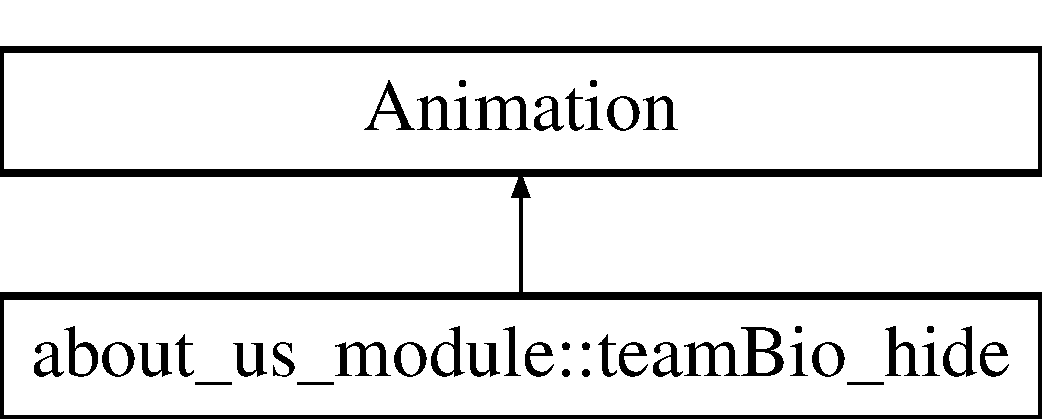
\includegraphics[height=2.000000cm]{classabout__us__module_1_1teamBio__hide}
\end{center}
\end{figure}


The documentation for this class was generated from the following file\-:\begin{DoxyCompactItemize}
\item 
about-\/us.\-js\end{DoxyCompactItemize}

\hypertarget{classexample__module_1_1teamBio__hide}{\section{example\-\_\-module\-:\-:team\-Bio\-\_\-hide Class Reference}
\label{classexample__module_1_1teamBio__hide}\index{example\-\_\-module\-::team\-Bio\-\_\-hide@{example\-\_\-module\-::team\-Bio\-\_\-hide}}
}
Inheritance diagram for example\-\_\-module\-:\-:team\-Bio\-\_\-hide\-:\begin{figure}[H]
\begin{center}
\leavevmode
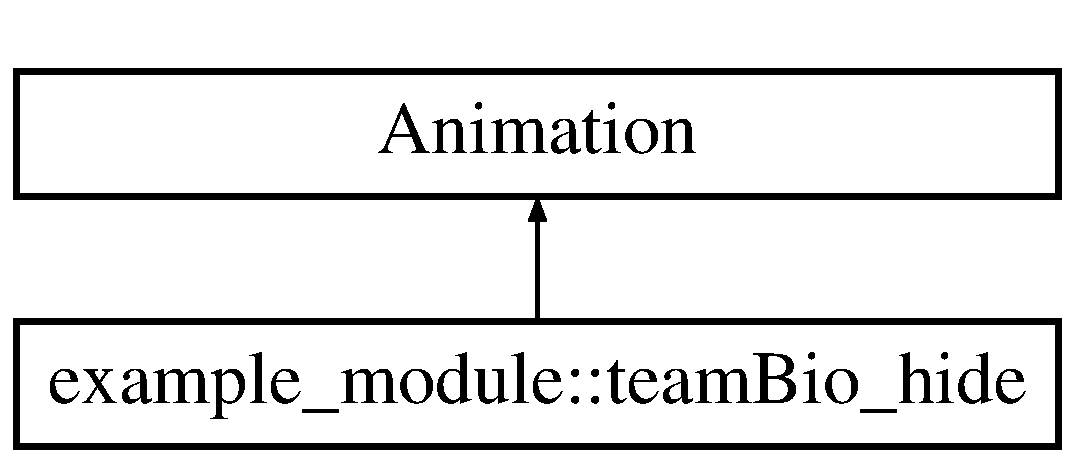
\includegraphics[height=2.000000cm]{classexample__module_1_1teamBio__hide}
\end{center}
\end{figure}


\subsection{Detailed Description}
animations and stuffz 

The documentation for this class was generated from the following file\-:\begin{DoxyCompactItemize}
\item 
example.\-js\end{DoxyCompactItemize}

\hypertarget{classabout__us__module_1_1teamBio__show}{\section{about\-\_\-us\-\_\-module\-:\-:team\-Bio\-\_\-show Class Reference}
\label{classabout__us__module_1_1teamBio__show}\index{about\-\_\-us\-\_\-module\-::team\-Bio\-\_\-show@{about\-\_\-us\-\_\-module\-::team\-Bio\-\_\-show}}
}
Inheritance diagram for about\-\_\-us\-\_\-module\-:\-:team\-Bio\-\_\-show\-:\begin{figure}[H]
\begin{center}
\leavevmode
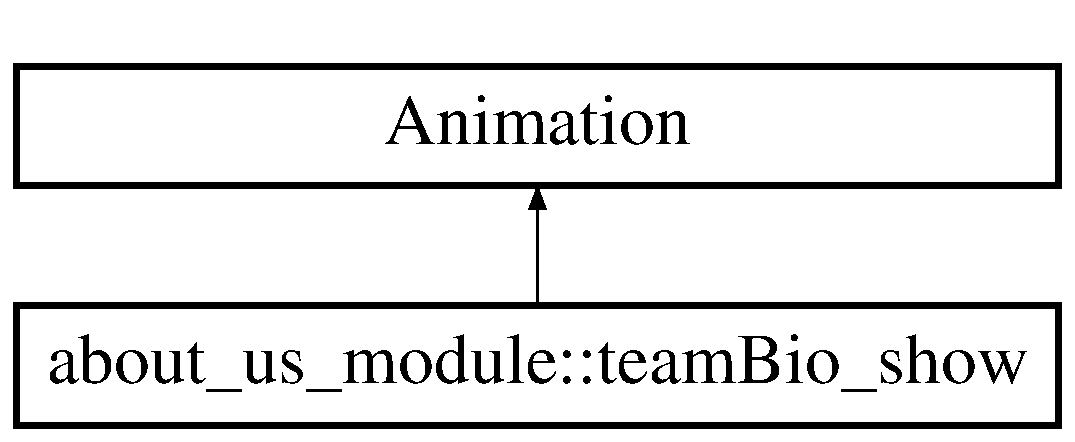
\includegraphics[height=2.000000cm]{classabout__us__module_1_1teamBio__show}
\end{center}
\end{figure}


The documentation for this class was generated from the following file\-:\begin{DoxyCompactItemize}
\item 
about-\/us.\-js\end{DoxyCompactItemize}

\hypertarget{classabout__us__module_1_1teamBioController}{\section{about\-\_\-us\-\_\-module\-:\-:team\-Bio\-Controller Class Reference}
\label{classabout__us__module_1_1teamBioController}\index{about\-\_\-us\-\_\-module\-::team\-Bio\-Controller@{about\-\_\-us\-\_\-module\-::team\-Bio\-Controller}}
}
Inheritance diagram for about\-\_\-us\-\_\-module\-:\-:team\-Bio\-Controller\-:\begin{figure}[H]
\begin{center}
\leavevmode
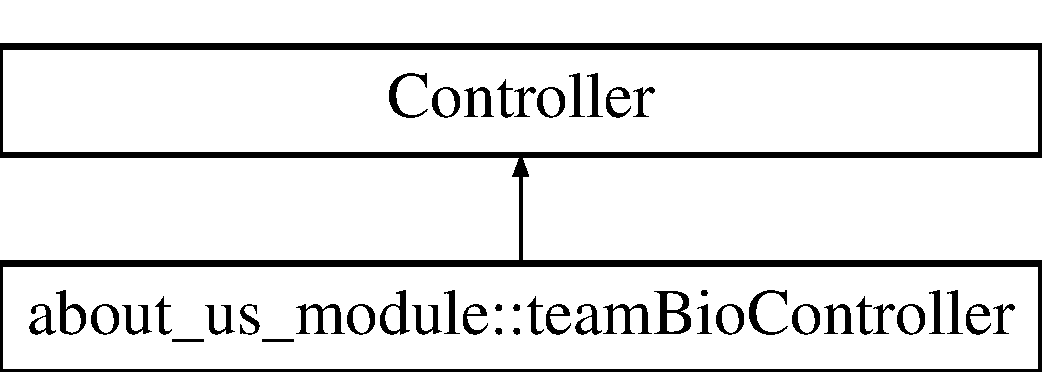
\includegraphics[height=2.000000cm]{classabout__us__module_1_1teamBioController}
\end{center}
\end{figure}
\subsection*{Public Attributes}
\begin{DoxyCompactItemize}
\item 
\hypertarget{classabout__us__module_1_1teamBioController_a559070080670303b17b2aa55cdd8b5fe}{{\bfseries team\-Members}}\label{classabout__us__module_1_1teamBioController_a559070080670303b17b2aa55cdd8b5fe}

\end{DoxyCompactItemize}


The documentation for this class was generated from the following file\-:\begin{DoxyCompactItemize}
\item 
about-\/us.\-js\end{DoxyCompactItemize}

\hypertarget{classabout__us__module_1_1teamMemberFactory}{\section{about\-\_\-us\-\_\-module\-:\-:team\-Member\-Factory Class Reference}
\label{classabout__us__module_1_1teamMemberFactory}\index{about\-\_\-us\-\_\-module\-::team\-Member\-Factory@{about\-\_\-us\-\_\-module\-::team\-Member\-Factory}}
}


\subsection{Detailed Description}
team\-Member factory makes teammembers of awesome.

{\itshape {\bfseries W\-A\-R\-N\-G\-I\-N\-G!} No interface could be parsed from this class. This could indicate a programming error. } 

The documentation for this class was generated from the following file\-:\begin{DoxyCompactItemize}
\item 
about-\/us.\-js\end{DoxyCompactItemize}

%--- End generated contents ---

% Index
\newpage
\phantomsection
\addcontentsline{toc}{part}{Index}
\printindex

\end{document}
